%"###############################################
%
% Classification supervisée
%
%###############################################

% RTUPB: prévision du profil de guérison
%
%###############################################

Nous utilisons ici la même méthode pour inférer arbres de régression et forêt aléatoire que lors de l'étude de prévision IPSS à 12 mois. A partir de l'arbre de régression complet obtenu sur l'échantilon d'apprentissage, la courbe évaluant le gain à chaque embranchement de l'arbre, figure~\ref{fig-rtupb-regtree-optim-healing-class} est quasi linéaire. Nous conservons donc cet arbre tel quel, sans élagage (figure~\ref{fig-rtupb-regtree-healing-class}.

\begin{figure}[H]
\centering
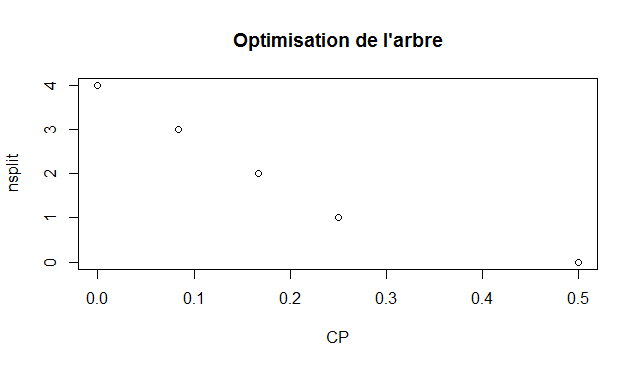
\includegraphics[width=0.75\textwidth]{../Fig/RTUPB/rtupb-regtree-optim-healing-class.png}
\caption{RTUPB: Arbre de régression pour profil de guérison}
\label{fig-rtupb-regtree-optim-healing-class}
\end{figure}

\begin{figure}[H]
\centering
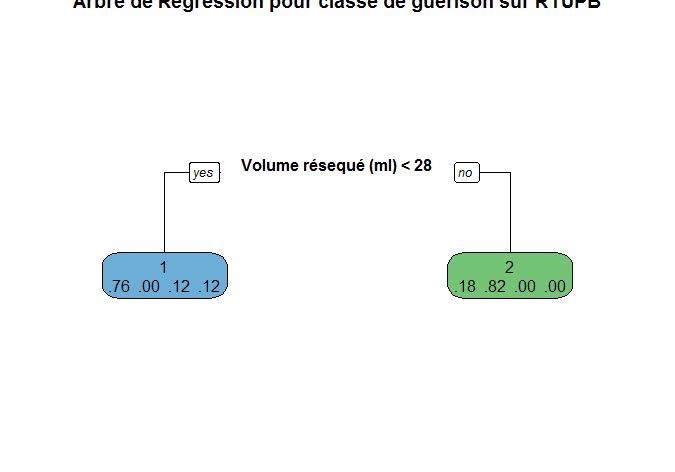
\includegraphics[width=0.75\textwidth]{../Fig/RTUPB/rtupb-regtree-healing-class.png}
\caption{RTUPB: Arbre de régression pour profil de guérison}
\label{fig-rtupb-regtree-healing-class}
\end{figure}

En appliquant l'arbre de régression sur l'échantillon de validation, nous obtenons des prévisions plutôt sûres d'elles (probabilité de 100\%) comme illustré figure~\ref{fig-rtupb-predict-healing-class}.

\begin{figure}[H]
\centering
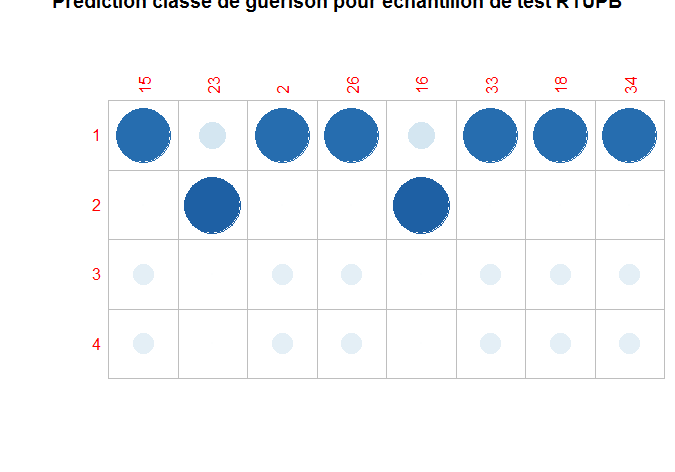
\includegraphics[width=0.75\textwidth]{../Fig/RTUPB/rtupb-predict-healing-class.png}
\caption{RTUPB: Prédiction du profil de guérison}
\label{fig-rtupb-predict-healing-class}
\end{figure}

En comparant plus objectivement les prédictions avec les profils effectifs des patients de l'ensemble de validation, nous constatons, ci-dessous, un taux d'erreur de 12,5\%.

\begin{lstlisting}[language=R]
          prediction
validation 1 2 3 4
         1 5 0 0 0
         2 1 1 0 0
         4 0 0 0 1
\end{lstlisting}

En utilisant une forêt aléatoire construite sur l'ensemble d'apprentissage, nous constatons alors, ci-dessous, un taux d'erreur de 0\%. La classification des profils pré-opératoires, s'avère donc fiable pour recommander une indication d'opération RTUPB et le profil de guérison associé.

\begin{lstlisting}[language=R]
          prediction
validation 1 2 3 4
         1 5 0 0 0
         2 0 2 0 0
         4 0 0 0 1
\end{lstlisting}


